\section{Strukturiertes Gitter}
Im Folgenden wird beschrieben, wie das strukturierte Netz der Aachen-Turbine erstellt wurde. Da das Netz die numerische Konvergenz der Lösungsverfahren, Qualität der Lösung, Auflösung und damit auch den Diskretisierungsfehler beeinflusst, ist ein gutes Netz von großer Bedeutung. Deshalb wurde eine Netzstudie - basierend auf einem Referenzgitter – durchgeführt und anschließend das bestmögliche Netz in Bezug auf Qualität vs. Rechenaufwand ausgewählt. Es war außerdem im Fokus, wie sich Netze unterschiedlicher Topologie hinsichtlich der erforderlichen Netzauflösung unterscheiden.

\subsection{Erstellung des Gitters}

Zunächst wurde das Referenzgitter erstellt. Dazu wurde die Geometrie der Aachen-Turbine mittels des strukturierten Multi-Block Netzgenerators AutoGrid5 vernetzt. Dieser ist speziell für die Vernetzung von Turbomaschinen ausgelegt. 
Das zur Verfügung stehende CAD-Modell der Aachen-Turbine die 1,5 Stufen zusammenhängend beinhaltete, wurden zu Beginn jeweils einzelne Gitter für Stator 1, Rotor und Stator 2 erzeugt, um diese später in CFX verwenden zu können. Hierbei wurde jeweils erst ein Vernetzungsdurchlauf basierend auf den voreingestellten Standardwerten durchgeführt und anschließend manuell optimiert. Für eine ausreichend gute Netzqualität dürfen bestimmte Netzkriterien nicht verletzt werden. Andernfalls kann es sein, dass der Diskretisierungsfehler steigt und die Lösung nicht oder nur schlecht konvergiert.
\begin{itemize}
	\item Keine negativen Kontrollvolumen
	\item Kleinster Winkel einer Zelle $> 20^\circ$
	\item Expasion ratio (Volumenverhältnis benachbarter Zellen) $< 3$
	\item Aspect ratio (Verhältnis längster zur kürzester Seite einer Zelle) $< 1000$ 
\end{itemize}
Variiert wurden die Anzahl und die Verteilung der Zellen in der S1-Ansicht. Diese stellt einen Querschnitt durch die Schaufel dar. In radialer Richtung wurde die Zellverteilung im „flowpath“ angepasst. 

\subsection{Spaltverfeinerung}

Zur Bestimmung der Gitterauflösung im Spalt des Rotors wurde zudem die Anzahl der Zellen im Spalt variiert. Es stellte sich heraus, dass im Vergleich zum ursprünglichen Gitter mehr Zellen hinzugefügt werden mussten, da die Auflösung nicht fein genug war und Änderungen, wie z.B. Spaltwirbel im Vergleich zur gröberen Auflösung nicht aufgelöst wurden. In den Abbildungen \ref{effSpalt1} und \ref{effSpalt15} ist die Gitterstudie für den Spalt mit 1 und 1,5 Stufen dargestellt. Als Ergebnis der Spaltverfeinerung wurde festgestellt, dass das Gitter mit der dreifachen Verfeinerung des ursprünglichen Spalts geeignet ist, da kaum noch ein Unterschied zum nächst feineren Gitter zu sehen ist und die Zellenanzahl trotzdem nicht zu groß ist.


\begin{figure}[H]
	\centering
	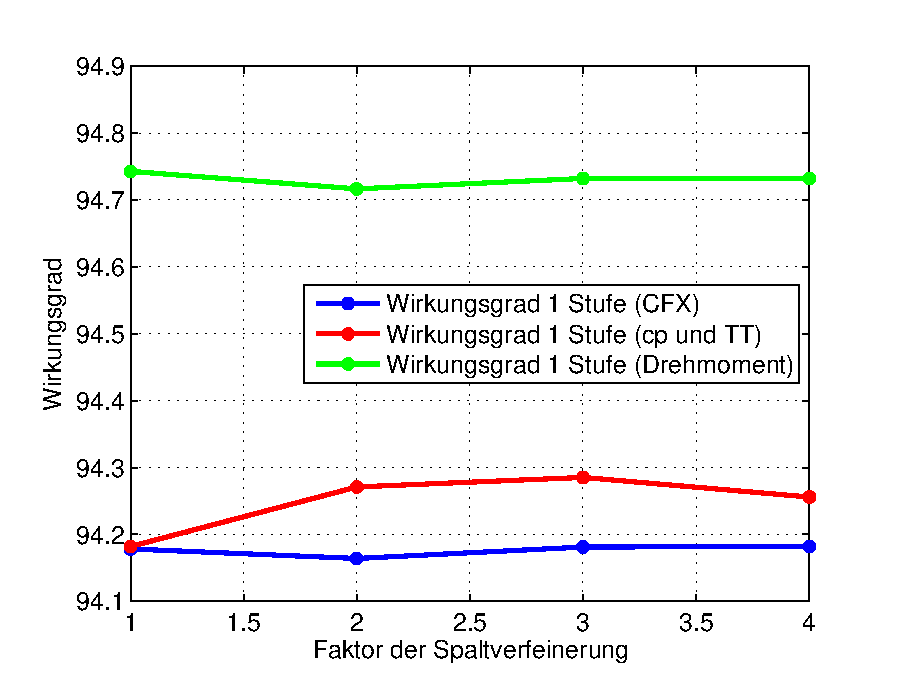
\includegraphics[width=0.7\textwidth]{efficiencySpalt1Stufe.eps}
	\caption{Gitterstudie des Spalts für eine Stufe} \label{effSpalt1}
\end{figure}

\begin{figure}[H]
	\centering
	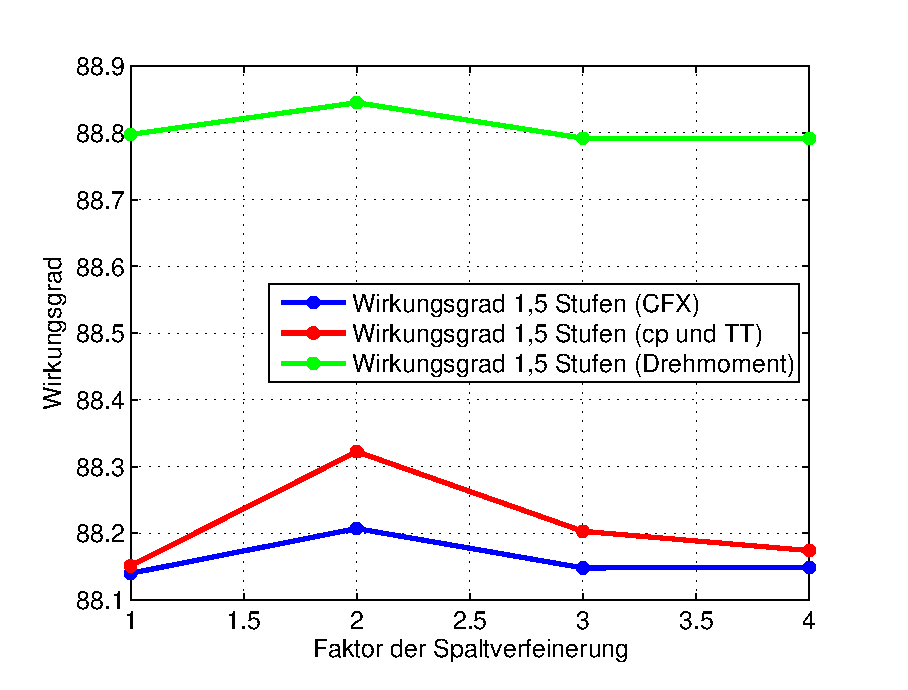
\includegraphics[width=0.7\textwidth]{efficiencySpalt15Stufen.eps}
	\caption{Gitterstudie des Spalts für 1,5 Stufen} \label{effSpalt15}
\end{figure}

\subsection{Einstellen der Grenzschichtdicke}
Der dimensionslose Wandabstand $y^+$ wurde iterativ bestimmt. Um das korrekte $y^+$ zu bestimmen, wurden die Werte in AutoGrid für den Wandabstand sowohl auf der Schaufeloberfläche im S1-Layer, als auch an Nabe und Gehäuse variiert.  Nach Bestimmen des Wandabstandes wurde eine Simulation in CFX durchgeführt und anschließend die Verteilung des $y^+$-Wertes über das Simulationsgebiet visualisiert und ausgewertet. Als finalen Wandabstand wurde für den Rotor $2\cdot 10^{-6}\text{m}$ im Flowpath an Nabe und Gehäuse und $1.5\cdot 10^{-6}\text{m}$ am Blade ermittelt. Ein Überblick der Werte ist in Tabelle \ref{cellWidths} zu sehen. Über das komplette Simulationsgebiet liegen die $y^+$-Werte in einem Bereich von $0.3 \leq y^+ \leq 3$. Da nur wenige Einstellparameter zur Beeinflussung dieses Wertes in AutoGrid vorhanden sind, ist dieser Wertebereich zufriedenstellend, zumal die Mehrheit der Werte im Bereich von $0.7 \leq y^+ \leq 1.2$  liegt, wie in Abb. \ref{imgYplusWerte} zu sehen ist. 

\begin{table}[H]
\centering
\begin{tabular}[t]{cccc}
\toprule
 Cell width in [m] & Stator1 & Rotor & Stator2  \\
\midrule
Cell width at Hub & $2.7e{-06}$ & $2e{-06}$ & $1.4e{-06}$\\
Cell width at Shroud & $2.7e{-06}$ & $2e{-06}$ & $1.4e{-06}$ \\
Cell width at Wall (Blade) & $1.56e{-06}$ & $1.5e{-06}$ & $1.7e{-06}$ \\
\bottomrule
\end{tabular}
\caption{Zellgrößen an der Wand für Rotor und die Statoren} \label{cellWidths}
\end{table}

\begin{figure}[H]
	\centering
    
	\includegraphics[width=0.7\textwidth]{yplus_final_2kk_finerGap3x.eps}
	\caption{$y^+$-Verteilung über die komplette Stufe} \label{imgYplusWerte}
\end{figure}

\subsection{Durchführung der Netzstudie}

Nachdem nun ein Referenzgitter mit guter Gitterqualität und korrekter Grenzschichtdicke vorhanden war, konnte die eigentliche Netzstudie durchgeführt werden um die minimale Auflösung zu bestimmen, die das Netz haben muss, damit die Lösung netzunabhängig ist. Hierzu wurden verschiedene Verfeinerungsstufen erstellt und dann der Einfluss auf verschiedene Größen, wie z.B. die Wirkungsgrade verglichen. Sobald sich der Wirkungsgrad im Vergleich zum nächst feineren, bzw. nächst gröberen Gitter kaum noch ändert, ist die Lösung von der Gitterdiskretisierung unabhängig. 
Insgesamt wurden 7 verschiedene Verfeinerungsstufen erstellt und simuliert, siehe Tabelle \ref{tab:Gittergroessen}. Das Referenzgitter hat jeweils circa 1 Million Zellen für Rotor und die Statoren. Zunächst wurde versucht, die Zellenanzahl zu verdoppeln. Dazu wurde die Auflösung in allen drei Raumrichtungen mit $\sqrt[3]{2}$ multipliziert um insgesamt einen Faktor von 2 zu erlangen. Dies wurde noch einmal wiederholt, um einen Faktor 4 der Gitterzellenanzahl gegenüber dem Referenznetz zu erreichen. Außerdem wurde das Referenznetz auf die halbe Zellenanzahl reduziert. Wie in den Abbildungen \ref{fig:efficiencies1strukturiert} und  \ref{fig:efficiencies15strukturiert} zu erkennen ist, ist die Lösung mit der doppelten Auflösung und etwa 7 Millionen Elementen praktisch netzunabhängig, sodass dieses als Referenzgitter für die nachfolgenden Rechnungen verwendet wird. 
In Tabelle \ref{tab:KenngroessenGitterFinal}  sind die Kenngrößen minimaler Winkel, maximales Aspect Ratio und maximales Expansion Ratio des finalen Gitters aufgelistet.

\begin{table}[H]
\centering
\begin{tabular}[t]{ccccc}
\toprule
Gittergröße	& Stator1 Knoten &	Stator1 Elemente & 	Rotor Knoten &	Rotor Elemente  \\
\midrule

0,5x 	& 593952	& 570112 &	830956	& 792464 \\
1,0x   &	995976	& 957440	&1379852	& 1324400\\
1,3x	  & 1337136	&1290344	&1279452	&1223280\\
1,5x 	&1440756	&1389568	&2640396	&2566336\\
\textbf{2,0x  }	&\textbf{2169132}	&\textbf{2105143}	&\textbf{3182040}&	\textbf{3099072}\\
3,0x  	&3484116	&3385344&	5498328	&5380440\\
4,0x 	& 3871240 &	3763968	&4538526&	4411680\\

\bottomrule
\end{tabular}

\begin{tabular}[t]{ccccc}
\toprule
Gittergröße	& Stator2 Knoten &	Stator2 Elemente & 	Globale Knoten &	Globale Elemente  \\
\midrule
0,5x 	& 532968	& 510016 &	1957876	& 1872592 \\
1,0x   &	977316	& 943296	&3353144	& 3225136 \\
1,3x	  & 1304928	&1259904	&3921516	&3773528\\
1,5x 	&1379992	&1330560	&5461144	&5286464\\
\textbf{2,0x  }	&\textbf{2500500}	&\textbf{2430400}	&\textbf{7851672}&	\textbf{7634615}\\
3,0x  	&4011168	&3913280&	12993612	&12679064\\
4,0x 	& 4267200 &	4164848	&12676966&	12340496\\

\bottomrule
\end{tabular}
\caption{Variationen der Gitter mit Knoten und Elementen} \label{tab:Gittergroessen}
\end{table}

\begin{table}[H]
\centering


\begin{tabular}[t]{cccc}
\toprule
Kenngröße	& Stator1 & Rotor &	Stator2  \\
\midrule
Min.Winkel [°]	& 29.25	& 25.75 & 36.10 \\
Max. Asp. Ratio   &	714.51	& 888.64	& 933.67 \\
Max. Exp. Ratio	  & 1.61	& 3.00	&1.80 \\


\bottomrule
\end{tabular}
\caption{Kenngrößen des finalen Gitters} \label{tab:KenngroessenGitterFinal}
\end{table}


\begin{figure}[H]
	\centering
	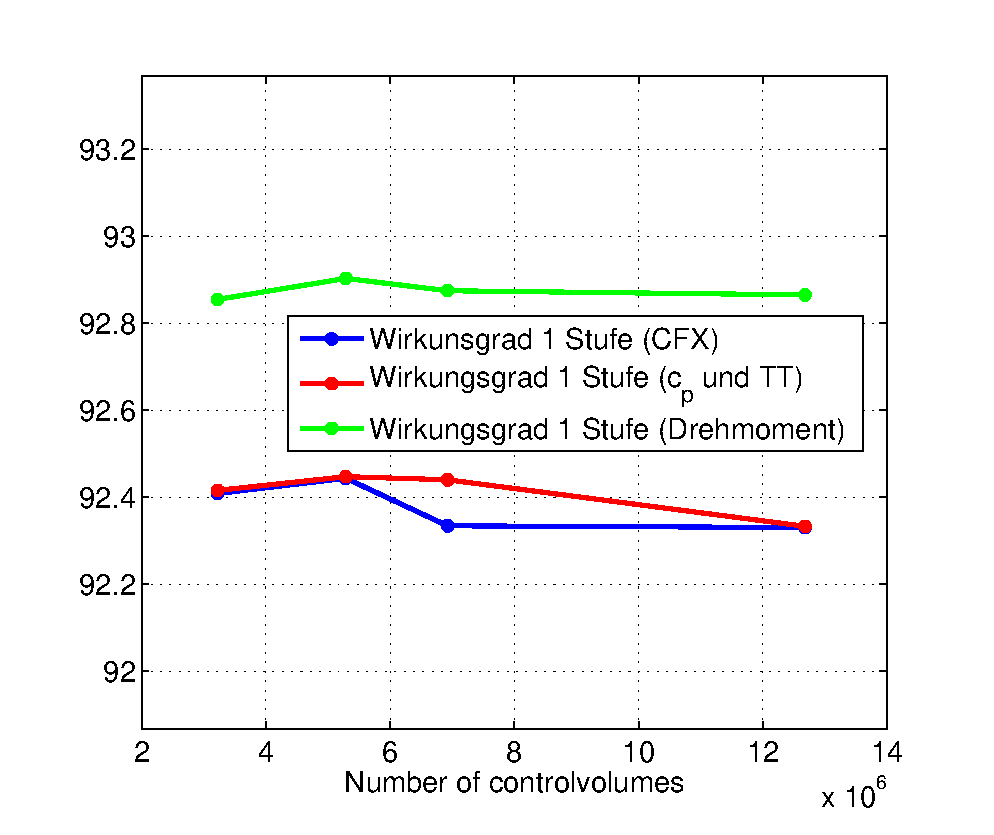
\includegraphics[width=0.7\textwidth]{efficiencies1strukturiert}
	\caption{Wirkungsgrade über eine Stufe} \label{fig:efficiencies1strukturiert}
\end{figure}

\begin{figure}[H]
	\centering
	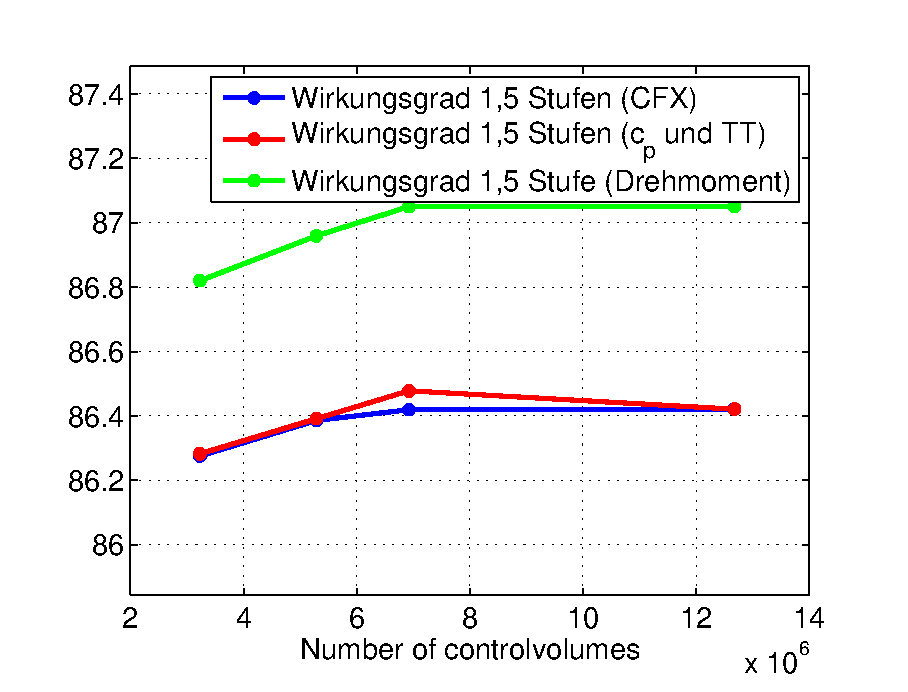
\includegraphics[width=0.7\textwidth]{efficiencies15strukturiert}
	\caption{Wirkungsgrade über 1,5 Stufen} \label{fig:efficiencies15strukturiert}
\end{figure}


\subsection{Fillets}

In realen Turbinen befinden sich an der Schaufel am Übergang zum Randbereich fertigungsbedingte Fillets, Verrundungen, um Ablöseblasen zu vermeiden und bessere Strömungs- und Festigkeitseigenschaften zu erzielen. Da außerdem die Qualität der Zellen am Übergang zur Nabe sehr schlecht war, wurde noch eine Simulation der Aachen-Turbine mit Fillets durchgeführt. Das Netz ist in Abb. \ref{imgFillet1} zu sehen. Jedoch ergab sich das Problem, dass nur sehr kleine Fillets erstellt werden konnten, da die Statoren eine „Delle“ an der Vorderkante aufweisen, wie in Abb. \ref{imgFilletDelle} zu sehen ist und daher ab einem bestimmten Filletradius negative Kontrollvolumen durch die Fillets entstehen. Deswegen wurde eine Simulation mit einem Fillet des Radius 0.00055 durchgeführt. Es hat sich herausgestellt, dass die Gitterqualität wesentlich schlechter wurde, da sich mehr schrägwinklige Zellen im Filletbereich befanden. Allerdings wurde der $y^+$-Wertebereich besser, da sehr kleine und sehr große Werte verschwanden.     

  \begin{figure}[H]
	\centering
	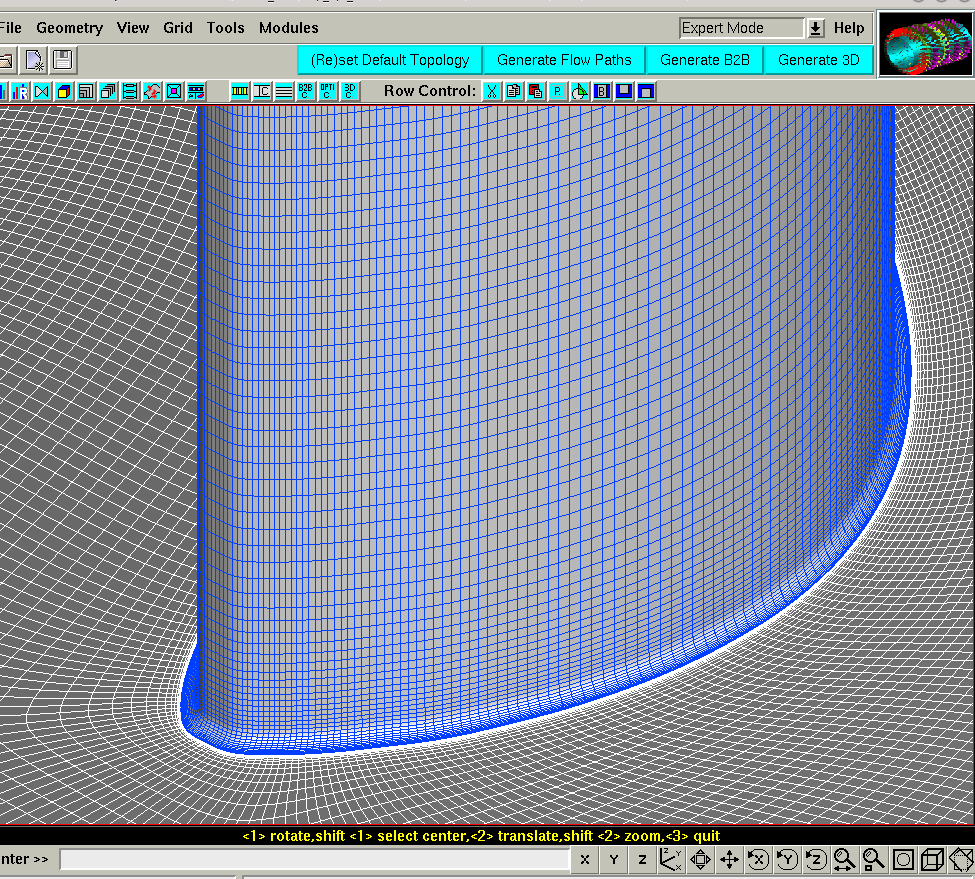
\includegraphics[width=0.7\textwidth]{fillet0_00055.png}
	\caption{Netz mit Fillet der Größe 0.00055} \label{imgFillet1}
\end{figure} 

  \begin{figure}[H]
	\centering
	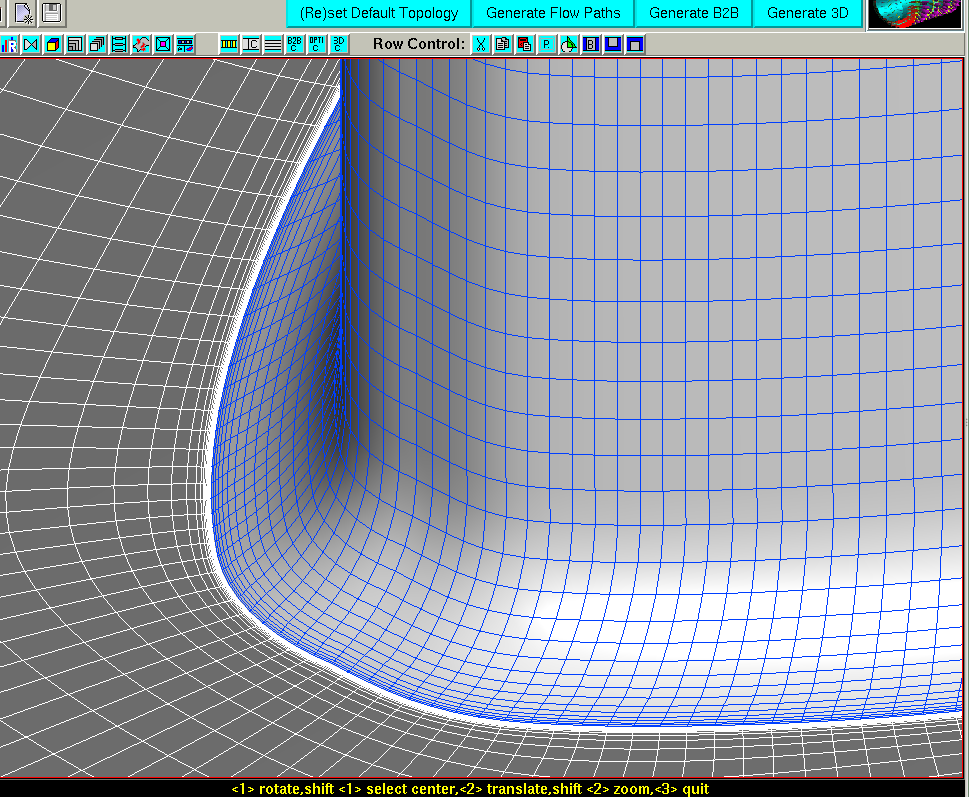
\includegraphics[width=0.7\textwidth]{filletDelle.png}
	\caption{Delle in der Statorgeometrie} \label{imgFilletDelle}
\end{figure} 